\documentclass[tikz]{standalone}
% \usepackage{pgfplots}
% \pgfplotsset{compat=1.18}
\usepackage{tkz-euclide}

\begin{document}
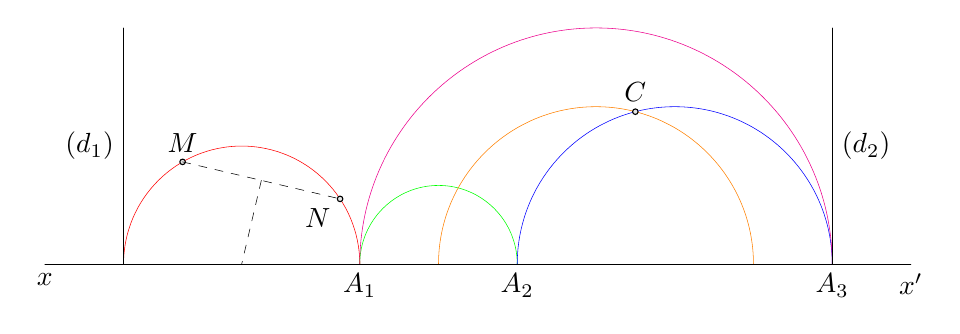
\begin{tikzpicture}
    % \tkzInit[xmin=-2, xmax=10, ymin=-1, ymax=3]
    \tkzDefPoints{-1/0/x1, 10/0/x2, 0/0/O, 3/0/A1, 5/0/A2, 9/0/A3}
    \tkzDefPoints{1.5/0/I1, 4/0/I2, 7/0/I3}
    \tkzDefPoints{0/3/B1, 9/3/B2}
    \tkzDefPoints{0.75/1.299/M, 2.75/0.829/N}
    \tkzDefPoints{6/0/U, 4/0/V1, 8/0/V2}
    \tkzDefMidPoint(A1,A3)\tkzGetPoint{S}
    \tkzDefMidPoint(M,N)\tkzGetPoint{P}
    \tkzInterCC(I3,A3)(U,V2)\tkzGetPoints{C1}{C2}

    % \tkzDrawY
    \tkzDrawArc[red](I1,A1)(O)
    \tkzDrawArc[green](I2,A2)(A1)
    \tkzDrawArc[blue](I3,A3)(A2)
    \tkzDrawArc[magenta](S,A3)(A1)
    \tkzDrawArc[orange](U,V2)(V1)
    \tkzDrawSegment(x1,x2)
    \tkzLabelPoint(x1){$x$}
    \tkzLabelPoint(x2){$x'$}
    \tkzDrawSegment(O,B1)
    \tkzDrawSegment(A3,B2)
    \tkzDrawPoints(M, N)
    \tkzDrawPoints(C2)
    \tkzDrawSegments[dashed](M,N P,I1)

    \tkzLabelPoint[below](A1){$A_1$}
    \tkzLabelPoint[below](A2){$A_2$}
    \tkzLabelPoint[below](A3){$A_3$}
    \tkzLabelPoint[above](M){$M$}
    \tkzLabelPoint[below left](N){$N$}
    \tkzLabelPoint[above](C2){$C$}
    \tkzLabelSegment[left](O,B1){$(d_1)$}
    \tkzLabelSegment[right](A3,B2){$(d_2)$}
% \begin{axis}[
%     axis lines=middle,
%     % xlabel=$x$,
%     % ylabel=$y$,
%     ymin=0, ymax=4,
%     xmin=-3, xmax=5,
%     xtick=\empty,
%     ytick=\empty,
%     axis line style={thick},
%     axis line style={->},
%     clip=false,
%     width=12cm,
%     height=8cm
% ]

% % Boundary line xx' (the x-axis)
% \draw[ultra thick, red] (axis cs: -3,0) -- (axis cs: 5,0);
% \node[red, below] at (axis cs: 4,0) {$xx'$};

% % Non-Euclidean plane background
% \fill[gray!10] (axis cs: -3,0) rectangle (axis cs: 5,4);

% % Hyperbolic lines (vertical lines)
% \draw[blue, thick] (axis cs: 1,0) -- (axis cs: 1,4);
% \draw[blue, thick] (axis cs: 3,0) -- (axis cs: 3,4);

% % Hyperbolic lines (semicircles)
% % Semicircle centered at (2,0) with radius 1.5
% \draw[blue, thick] (axis cs: 0.5,0) arc (180:0:1.5);
% % Semicircle centered at (-1,0) with radius 1
% \draw[blue, thick] (axis cs: -2,0) arc (180:0:1);

% % Points and labels
% \node[circle,fill=black,label=above left:$P$] at (axis cs: 1,2) {};
% \node[circle,fill=black,label=above left:$Q$] at (axis cs: 3.5,1.5) {};

% % Example geodesic between P and Q
% \draw[red, dashed, thick] (axis cs: 1,2) arc (180:-20:1.25);

% % Center markers (not part of the model)
% \draw[dashed, gray] (axis cs: 2,0) -- (axis cs: 2,0.5);
% \draw[dashed, gray] (axis cs: -1,0) -- (axis cs: -1,0.5);

% % Legend
% % \node[blue, right] at (axis cs: 4,3.5) {Hyperbolic lines:};
% % \node[blue, right] at (axis cs: 4,3) {-- Vertical lines};
% % \node[blue, right] at (axis cs: 4,2.5) {-- Semicircles centered on $xx'$};
% % \node[red, right] at (axis cs: 4,2) {Boundary $xx'$};
% % \node[red, right] at (axis cs: 4,1.5) {Geodesic between $P$ and $Q$};

% \end{axis}
\end{tikzpicture}
\end{document}